\section{The door in the full collapse}\label{sec:door}

The witness of Section~\ref{sec:witness} lives in the linear chain. The question it leaves is whether hidden angular structure that density, flux and stress do not carry can move the black-hole threshold itself, in the full general-relativistic collapse. This section answers it with McCormick's code.

\paragraph{The construction.} Run the gradual-decoupling Gaussian case ($R_\nu=0.409$, $n=3$, $\epsilon_{\rm dec}=2$, $N=400$, $N_\mu=32$, one collision rate evaluated at every Runge--Kutta stage) to a restart surface $\epsilon_s$, landing on it exactly, and save the whole state. In every cell change only the hidden part of the angular intensity:
\begin{equation}
\delta I_{ik}=f\,b(r_i)\,m_i\,\frac{\varepsilon_i}{4\pi}\,p_\ell(\mu_k),
\end{equation}
where $p_\ell$ is the discrete orthogonal polynomial on the 32 angle bins (orthogonal to $1,\mu,\mu^2$ to $2\times10^{-17}$), $b$ a smooth bump that vanishes identically for $r\le0.3r_m$ and $r\ge2r_m$, $m_i$ the cell's positivity margin, and $f=\pm\tfrac12$. The bump keeps the perturbation regular at the centre, where a regular $\ell$-th moment must vanish like $r^\ell$; a perturbation uniform in radius is irregular there, and its first test moved the central neutrino density by $91\%$, so it was dropped as a verdict tool. Between the $+f$ and $-f$ states, at all three restart surfaces, the discrete $\ell=0,1,2$ components agree to $4.4\times10^{-16}$ of $c_0$; the energy, radial pressure and mass to $9\times10^{-16}$; the flux to $10^{-16}$ of the energy; the lapse to $2\times10^{-15}$; the constraint $\Gamma^2-(1+U^2-2M/R)$ to $7\times10^{-15}$; the fluid and metric arrays are bit-identical. The hidden component differs by $0.08$--$0.17$ of $c_0$ \grade{measured; Appendix~A.15}. To any fluid description, and to every quantity that enters Einstein's equations at the restart, the two states are the same state.

\paragraph{The readings, written down first.} The door of Section~\ref{sec:witness} predicts that structure planted at decoupling ($\epsilon_s=2$) moves the threshold and structure planted deep in the coupled era ($\epsilon_s=0.5$) does not. The opposite reading is that the nonlinear collapse washes out $\ell\ge3$ whatever the timing. A third restart surface, $\epsilon_s=4$, in free streaming, was added before any threshold run. A difference counts as real only if the two brackets, each widened by twice a measured resolution drift, stay apart; the drift, measured by rerunning the decoupling $\ell=3$ pair with $48$ angle bins, is $d_K=1.65\times10^{-4}$. No sign was predicted.

\paragraph{Eight thresholds.} The unperturbed restart at $\epsilon_s=2$ gives $\delta_c=0.5107500\pm0.0000093$, within one bracket of the $r=1$ threshold of Section~\ref{sec:link}. Each threshold below is found by trisection under the endpoint rule of Section~\ref{sec:link}:
\begin{center}\small\begin{tabular}{llccc}\toprule
$\epsilon_s$ & hidden direction & $\delta_c(+f)$ & $\delta_c(-f)$ & difference\\\midrule
$0.5$ & $\ell=3$ & $0.5107685$ & $0.5107510$ & $+1.75\times10^{-5}$\\
$0.5$ & $\ell=4$ & $0.5107685$ & $0.5107500$ & $+1.85\times10^{-5}$\\
$2$ & $\ell=3$ & $0.5125833$ & $0.5088395$ & $\mathbf{+3.744\times10^{-3}}$\\
$2$ & $\ell=3$, $N_\mu=48$ & $0.5125134$ & $0.5090041$ & $\mathbf{+3.509\times10^{-3}}$\\
$2$ & $\ell=4$ & $0.5096749$ & $0.5117726$ & $\mathbf{-2.098\times10^{-3}}$\\
$2$ & Gramian direction & $0.5134352$ & $0.5079300$ & $\mathbf{+5.505\times10^{-3}}$\\
$4$ & $\ell=3$ & $0.5108796$ & $0.5106358$ & $+2.44\times10^{-4}$\\
$4$ & $\ell=4$ & $0.5106759$ & $0.5108241$ & $-1.48\times10^{-4}$\\\bottomrule\end{tabular}\end{center}
Bracket widths are $0.8$--$1.85\times10^{-5}$ \grade{measured; Figure~\ref{fig:doornl}}. At decoupling all three directions are real: the differences are $202$, $204$ and $297$ bracket widths and survive the drift allowance with room. In the coupled era both agree within two bracket widths, as predicted. In free streaming the raw differences are $13$ and $8$ bracket widths with the decoupling signs, but they fall inside the drift allowance; by the rule written first they are not called real. The opposite reading is excluded by the decoupling pairs.

\paragraph{What the collapse reads.} Odd hidden structure oriented like $+p_3$ raises the threshold, by $+1.83\times10^{-3}$ from the unperturbed restart, and $-p_3$ lowers it by $1.91\times10^{-3}$: the response is close to odd in the amplitude. Even structure works the other way: $+p_4$ lowers the threshold, at $0.56$ of the $p_3$ size (the linear Gramian gave $0.40$). The Gramian direction of Section~\ref{sec:gramian} moves the threshold $1.47$ times as much as pure $p_3$ at the same positivity margin, in the same direction: the predictive-quotient ranking of hidden directions carries into the nonlinear collapse, at about $60\%$ of its linear size. For scale, the decoupling difference of $3.5\times10^{-3}$ is $11\%$ of McCormick's whole free-streaming shift, $0.49773\to0.52832$, and ten times the flux--shear link effect in his physical model (Section~\ref{sec:mcc}).

\paragraph{The coupled era is not perfectly shut.} At $\epsilon_s=0.5$ the paired runs still separate in compaction by $10^5$ times their noise floor, and the separation does not fall with angular refinement ($48$ against $32$ bins: ratio $0.86$--$0.89$, where an angular-grid leak would fall to about $0.44$). It is a channel of the general-relativistic solver, and it carries about $0.3$--$0.5\%$ of the decoupling effect, where the linear survival factor gives $5\times10^{-10}$. The witness chain has no such channel; a candidate, untested, is the fluid-frame shear and acceleration terms, which couple $\ell=3$ to $\ell=2$ at a rate set by the shear of the flow rather than by $k$, so that the coupled-era suppression is about $S/\kappa$ per rung. Its dependence on radial resolution is untested.

\paragraph{Reading.} The door is a window centred on decoupling: shut in the coupled era to within a fraction of a per cent, open at decoupling, narrowing again in free streaming because structure planted late has too little time to stream back into density and stress before the collapse is decided, near $\epsilon\approx4$--$6$. The black-hole threshold reads angular information that no closure on density, flux and stress holds. This is an engineered sensitivity, at half each cell's positivity margin, on one profile: whether cosmological initial data carry such structure at decoupling is a separate question, not answered here \grade{H}.

\begin{figure}[t]\centering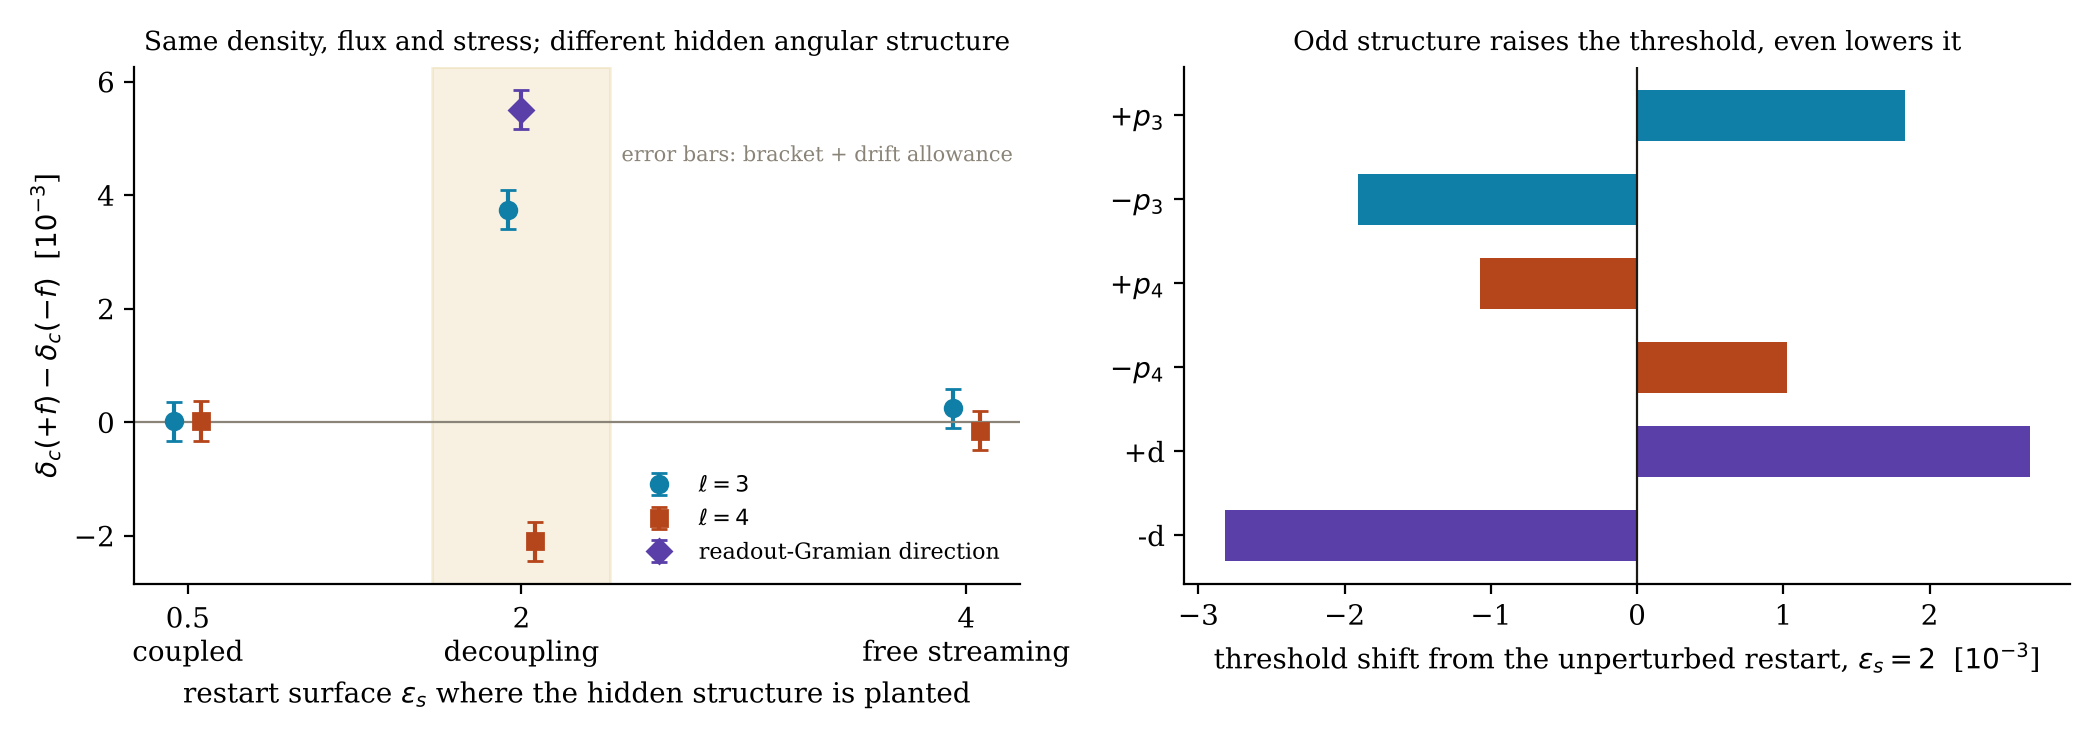
\includegraphics[width=\textwidth]{figs/fig8_door_nonlinear.png}
\caption{The door in the full collapse. Left: the difference in black-hole threshold between two neutrino states with identical density, flux, stress, energy, radial pressure, lapse and constraints, differing only in hidden angular structure, against the epoch at which the structure is planted; error bars are bracket half-widths plus twice the measured angular drift. Right: the threshold shifts from the unperturbed restart at decoupling.}\label{fig:doornl}\end{figure}
